\documentclass[12pt]{article}
\usepackage{amsmath}
\usepackage{amssymb}
\usepackage[letterpaper,margin=0.85in,centering]{geometry}
\usepackage{fancyhdr}
\usepackage{enumerate}
\usepackage{lastpage}
\usepackage{multicol}
\usepackage{graphicx}

\reversemarginpar

\pagestyle{fancy}
\cfoot{}
\lhead{Math 1560}\chead{Test \# 1}\rhead{May 18th, 2017}
%\rfoot{Total: 10 points}
%\chead{{\bf Name:}}
\newcommand{\points}[1]{\marginpar{\hspace{24pt}[#1]}}
\newcommand{\skipline}{\vspace{12pt}}
%\renewcommand{\headrulewidth}{0in}
\headheight 30pt

\newcommand{\di}{\displaystyle}
\newcommand{\abs}[1]{\lvert #1\rvert}
\newcommand{\len}[1]{\lVert #1\rVert}
\renewcommand{\i}{\mathbf{i}}
\renewcommand{\j}{\mathbf{j}}
\renewcommand{\k}{\mathbf{k}}
\newcommand{\R}{\mathbb{R}}
\newcommand{\aaa}{\mathbf{a}}
\newcommand{\bbb}{\mathbf{b}}
\newcommand{\ccc}{\mathbf{c}}
\newcommand{\dotp}{\boldsymbol{\cdot}}
\newcommand{\bbm}{\begin{bmatrix}}
\newcommand{\ebm}{\end{bmatrix}}                   
                  
\begin{document}
\thispagestyle{plain}
\begin{center}
{\bf MATH 1560 - Test 1}\\
Examiner: Sean Fitzpatrick
\end{center}
\skipline \skipline \skipline \noindent \skipline
Last Name:\underline{\hspace{350pt}}\\
\skipline
First Name:\underline{\hspace{348pt}}\\
\skipline
Student Number:\underline{\hspace{322pt}}\\
\skipline

%\author{Instructor: Sean Fitzpatrick}
\thispagestyle{fancy}
%\noindent{{\bf Name and student number:}}

 \begin{enumerate}
 \item  Evaluate the following limits:
\begin{enumerate}
 \item $\di \lim_{x\to 3} \frac{x^2-5x+6}{x^2-4x+3}$ \points{3}

\vspace{2in}

 \item $\di \lim_{x\to 0}\frac{\sin(5x)}{x}$ \points{3}

\vspace{2in}

 \item $\di \lim_{x\to 0}\left(\frac{1}{x}-\frac{1}{x^2+x}\right)$ \points{3} (Suggestion: common denominator.)

\end{enumerate}
\newpage

\item The graph of a function $f$ is given below:

\begin{center}
 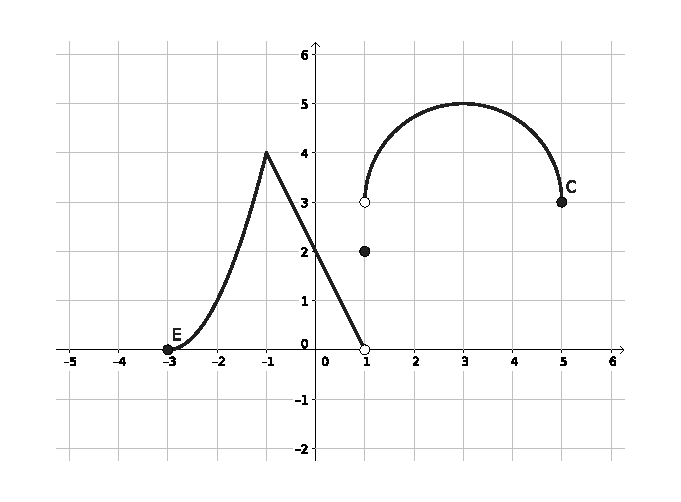
\includegraphics[width=5in]{TT1_fig1}
\end{center}

\begin{enumerate}
 \item What is the domain of $f$?\points{1}

\bigskip

\bigskip

 \item $\di\lim_{x \to -1^-}f(x)= $ \underline{\hspace{1in}} and $\di \lim_{x\to -1^+}f(x)= $ \underline{\hspace{1in}}  \points{1}

\bigskip

\bigskip


 \item $\di \lim_{x \to 1^-}f(x)=$ \underline{\hspace{1in}} and $\di \lim_{x\to 1^+}f(x) =$ \underline{\hspace{1in}} \points{1}

\bigskip

\bigskip

 \item On what interval(s) is $f$ continuous? \points{1}
\end{enumerate}

\bigskip

\bigskip

\item What are the horizontal and vertical asymptotes (if any) of $f(x) = \dfrac{\sqrt{x^2+1}}{x-1}$?\points{2}
\end{enumerate}





\end{document}